\chapter{Survey on Existing Techniques}
\label{chapter.Survey}
\markright {Survey on Existing Techniques}

\section{Introduction}

\section{Review of Path Computation Techniques for Interdomain LSPs}
Puype et al. [PUP03][YAN05] propose Multi-Layer Traffic Engineering (MTE) schemes based on two main strategies: a �reactive� one where MTE actions are triggered only by the detection of network congestion and a �proactive� one that tries to keep the network optimal at all times, triggering a reconfiguration whenever optimizations are possible.
Sabela et al. [SAB03] propose an offline multilayered solution for the global path provisioning in GMPLS multilayered optical networks. They propose a new heuristic and to solve an optimization problem with help of the CPLEX solver optimizing network configuration and traffic routing considering both the optical and the electrical layers.
Iovanna et al. [IOV03] propose a hybrid approach for the routing of IP/MPLS LSPs over a WDM layer which takes advantage of a combined use of off-line and on-line routing strategies to optimize the use of network resources. The proposed heuristic approach is composed of two main phases: (i) an initial paths set-up (performed off-line) by means of a successive shortest-path algorithm (ii) an on-line local search procedure (triggered by network congestion detection) based on the deletion of the lightest loaded lightpath and used for improving the resource utilization to allow the accommodation of incoming LSP requests. Compared to the previous scheme, no details are included here to describe when a link can be considered congested.

\section{Review of Protection and Restoration Techniques}
\subsection{Multi-layer Survivability}
Demeester et al. [DEM99] studied survivability in multi-layer transport networks. They provided guidelines for coordination of recovery actions in WDM, SONET, and ATM layers. Quantitative comparisons were given in terms of recovery time and investment cost. Fumagalli et al. [FUM00] also envisioned the cooperation of the IP and optical layers in providing network resiliency. A heuristic based on simulated annealing was proposed to choose the optimal protection/restoration scheme for each link of an IP-over-optical mesh network. Finally, the practical requirements for multi-layer survivability were examined in the recent RFC [LAI02], in which the use of nested hold-off timers was recommended.

\subsection{Multi-Domain Survivability}
As the network relies more on multiple carriers, issues of survivability in multi-domain/multi-area networks are becoming important in the IP-over-optical network community. Huang in [HUA02] introduced a set of mechanisms for establishing LSPs that span multiple routing areas. Papadimitriou et al. [PAP05] analyzed suitability of using the GMPLS control plane in multi-region networks. Finally, RFC 3386 [LAI02] studied interoperable survivability approaches in a multi-provider environment. Criteria that trigger protection mechanisms at domain boundaries, as well as requirements on the interaction of protection mechanisms on both sides of a boundary, were suggested.

\begin{figure}[t]
\centering
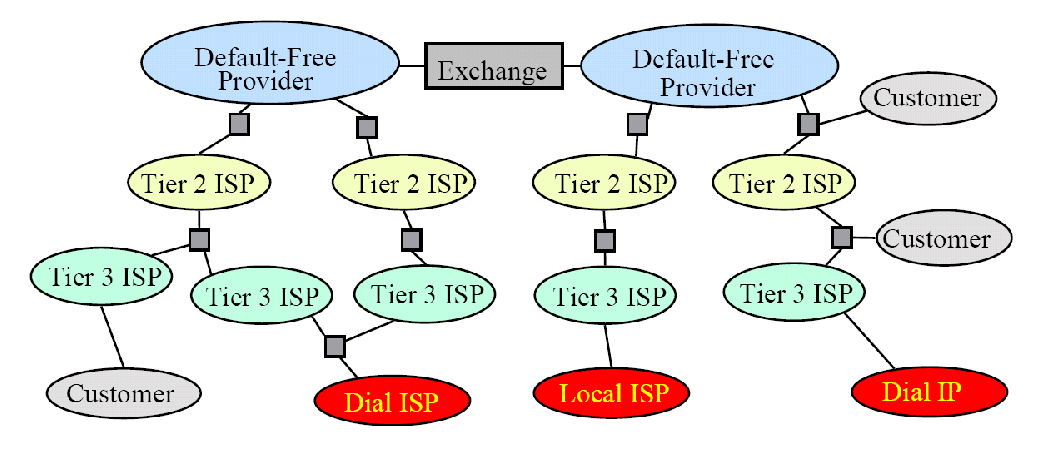
\includegraphics[scale=0.7]{Figures/InternetArchitecture.eps}
\caption{The Internet Architecture}
\label{fig:InternetArchitecture}
\end{figure}

\section{Review of PCE Selection Techniques}
\begin{itemize}
    \item Mesh of separate networks connected at exchange points
	 \item Tier 1 Providers carry full Internet Routing Tables � No defaults
	 \item Tier 2+ Providers carry subset and point to �upstream� default
\end{itemize}

What Is an Intranet?
� A small to global-size collection of interconnected computing resources
available to a closed set of end-users
- could be extended across shared, public Internet or ISP network via tunnels �
VPN
� Applications are distributed (e.g. e-mail) and centralized (e.g. mainframe)
� (Still) based on many protocols � IP, IPX, SNA, Decnet, etc.
- direction towards TCP/IP
� Performance MUST be predictable and Security is ASSUMED
� Internet technologies are now commonplace for corporate networkers
- Web Browser access to corporate resources (including the mainframe which is now just a big server)
- Secure mobile access with performance
- Internet access

\section{Conclusions}
